% This is LLNCS.DEM the demonstration file of
% the LaTeX macro package from Springer-Verlag
% for Lecture Notes in Computer Science,
% version 2.4 for LaTeX2e as of 16. April 2010
%
\documentclass{llncs}
%
\usepackage{makeidx}  % allows for indexgeneration
\usepackage[hidelinks]{hyperref}
\usepackage{graphicx}
\usepackage{listings}
\usepackage[utf8]{inputenc}
\usepackage[ngerman]{babel}

\hypersetup{
	pdftitle = {Objekt Algebra - Ein Lösungsansatz für das Expression Problem},
	pdfsubject = {Software-Development},
	pdfauthor = {Marco Buchholz, Max Golubew, Florian Winzek},
	pdfkeywords = {expression problem, visitor pattern, interpreter pattern, object algebra}, 
	colorlinks = false
}

%
\begin{document}
%
\frontmatter          % for the preliminaries
%
\pagestyle{headings}  % switches on printing of running heads
%
\mainmatter              % start of the contributions
%
\title{Objekt Algebra - Ein Lösungsansatz für das Expression Problem}
%
\titlerunning{Objekt Algebra - Ein Lösungsansatz für das Expression Problem}  % abbreviated title (for running head)
%                                     also used for the TOC unless
%                                     \toctitle is used
%
\author{Marco Buchholz%\inst{1}%\orcidID{0000-1111-2222-3333}
\and
Max Golubew%\inst{2}%\orcidID{1111-2222-3333-4444} 
\and
Florian Winzek%\orcidID{2222-3333-4444-5555}
}
%
\authorrunning{Marco Buchholz, Max Golubew, Florian Winzek} % abbreviated author list (for running head)
%
%%%% list of authors for the TOC (use if author list has to be modified)
\tocauthor{Marco Buchholz, Max Golubew, Florian Winzek}
%
\institute{Institute for Software Engineering and Programming Languages, Universität zu Lübeck\\
\email{marco.buchholz@student.uni-luebeck.de} \\
\email{max.golubew@student.uni-luebeck.de} \\
\email{f.winzek@student.uni-luebeck.de}}

\maketitle              % typeset the title of the contribution

\begin{abstract}
Das Expression Problem ist ein bekanntes Problem in der Funktionalen Programmierung. Hierbei geht es darum, dass ein Programm, welches aus Datenstrukturen und Funktionen besteht, in diese zwei Dimensionen weiterentwickelt werden soll, ohne das Programm neu kompilieren zu müssen. Die Komplexität des Programs darf ebenfalls nicht größer werden. In diesem Paper behandeln wir einen Ansatz, welcher das Problem lösen kann. In diesem Zusammenhang stellen wir das Konzept der Objekt Algebra. Wir werden Lineare Zeit Logik Formeln (LTL-Formeln) als anschauliches Beispiel benutzen. Um zu zeigen, dass die Objekt Algebra ein Programm auf einfache Art um Operationen und Datenstrukturen weiterentwickeln kann, werden wir zunächst eine Grundmenge von LTL-Formeln betrachten und diese dann um zusätzliche Formeln und Funktionen erweitern.

\end{abstract}
%
\section{Einleitung} \label{sec:introduction}

Beim Expression Problem geht es speziell um Computerprogramme oder Algorithmen. Diese werden im Laufe der Entwicklung immer komplexer. Das bedeutet, es kommen neue Funktionen für bestehende Datentypen hinzu, aber auch neue Datentypen für aktuelle Funktionen. Diese beiden Dimensionen sollten beim Entwicklungsprozess möglichst dynamisch gehalten werden, damit das Programm nicht zu komplex wird. Oftmals muss der Code neu geschrieben und kompiliert werden. 

Es gibt einige Ansätze um zumindest einen der zwei Dimensionen dynamisch weiterzuentwickeln. Wir werden im folgenden Kapitel auf diese Ansätze eingehen und die Vor- und Nachteile erörtern. Im Anschluss stellen wir einen alternativen Ansatz vor, welcher beide Dimensionen gleichzeitig abdeckt. Zum Schluss zeigen wir eine mögliche Implementierung am Beispiel von LTL-Formeln.   

\section{Lösungsansätze} \label{sec:approaches}

In diesem Kapitel wollen wir zunächst ein wenig auf bekannte Software Pattern eingehen, die sich im Kern mit dem Expression Problem auseinandersetzen. Dies sind zum Einen das sogenannte \emph{Interpreter Pattern} und das \emph{Visitor Pattern}. Ein alternativer Ansatz stellt die sogennante \emph{Objekt Algebra} dar, auf welchen wir insbesondere eingehen werden. 

\subsection{Interpreter Pattern} \label{ssec:interpreter}

\subsection{Visitor Pattern} \label{ssec:visitor}

\subsection{Objekt Algebra} \label{ssec:oa}

\section{Implementation} \label{sec:implementation}
\begin{figure}
	\centering
	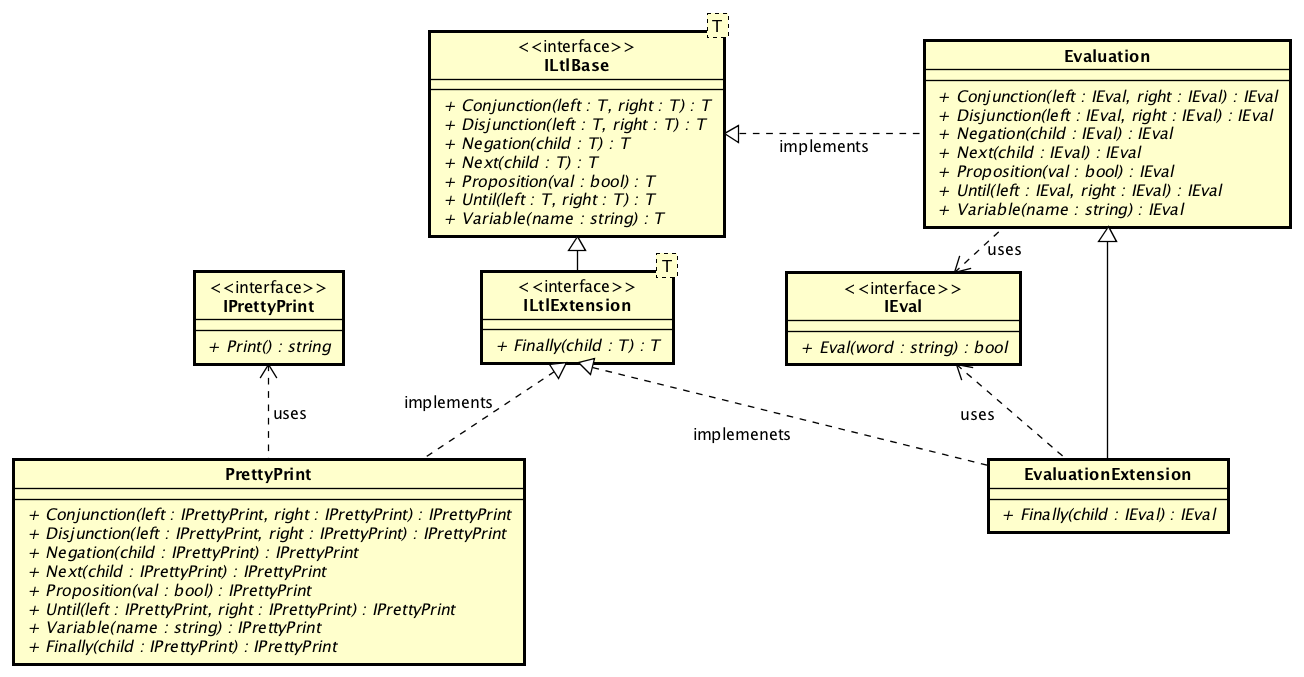
\includegraphics[width=\textwidth]{images/ObjectAlgebra.png}
	\caption{text}
	\label{fig:object-algebra}
\end{figure}

\section{Zusammenfassung} \label{sec:conclusion}


%
% ---- Bibliography ----
%
\begin{thebibliography}{5}
%

\bibitem{wadler98}
Wadler, P.:
The Expression Problem.
E-Mail Discussion (1998),
\url{http://homepages.inf.ed.ac.uk/wadler/papers/expression/expression.txt}

\bibitem{Odersky05}
Odersky, M., Zenger, M.:
Independently Extensible Solutions to the Expression Problem. 
In FOOL'05

\bibitem{pnueli77}
Pnueli, A.:
The temporal logic of programs.
In 18th Annual Symposium on Foundations of Computer Science, Providence, Rhode Island, USA, 31 October - 1 November 1977, pages 46-57, IEEE Computer Society, 1977

\bibitem{GHJV94}
Gamma, E., Helm R., Johnson R. and Vlissides J.:
Design Patterns: Elements of Reusable Object-Oriented Software.
Addison-Wesley Professional Computing Series, Pearson Education, 1994

\bibitem{Parr09}
Parr, T.:
Language Implementation Patterns: Create Your Own Domain-Specific and General Programming Languages.
Pragmatic Bookshelf, 2009

\bibitem{Oliveira12}
Oliveira, B., Cook, W.:
Extensibility for the Masses - Practical Extensibility with Object Algebras.
In ECOOP 2012 -- Object-Oriented Programming: 26th European Conference, Beijing, China, June 11-16, 2012, pages 2-27, Springer Berlin Heidelberg

\bibitem{Guttag78}
Guttag, J., Horning, J.:
The algebraic specification of abstract data types.
In Acta Informatica Vol. 10, pages 27-52, March 1978

\end{thebibliography}
\end{document}
